% !TEX TS-program = xelatex
% !TeX spellcheck = ru_RU
% !TEX root = cfg1.tex

\documentclass[tikz,border=3.14mm]{standalone}

\usepackage{fontspec}
\usepackage{euler-math}
\setmainfont[Ligatures=TeX]{Liberation Serif}
\setsansfont[Ligatures=TeX]{Liberation Sans}

\usetikzlibrary{chains,shadows.blur}
  \def\mynode#1#2 {
      \node[box] (b#1) {#2};
      \node [right,inner xsep=.5em
          , outer sep=0pt,text height=1ex,text depth=.0ex] (caption#1)
                   at ([shift={(-1em,0pt)}]b#1.north west) {#1};
  }
  \newcommand{\FixedLengthArrow}{2,0}
\begin{document}
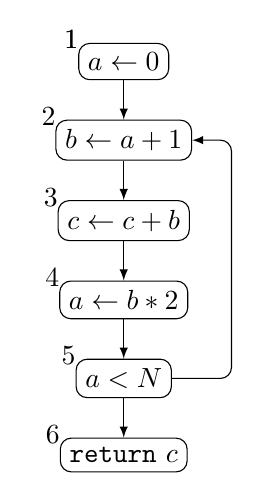
\begin{tikzpicture}[auto,
  node distance = 5mm,
  start chain = going below,
  box/.style = {draw,rounded corners
    %, blur shadow
    , fill=white
    , on chain,align=center}]

 \mynode{1}{$a\leftarrow0$}
 \mynode{2}{$b\leftarrow a+1$}
 \mynode{3}{$c\leftarrow c+b$}
 \mynode{4}{$a\leftarrow b*2$}
 \mynode{5}{$a<N$}
 \mynode{6}{\texttt{return} $c$}

 \node [right,inner xsep=.5em
    , outer sep=0pt,text height=1ex,text depth=.0ex] (ttt1)
             at ([shift={(-1em,0pt)}]b1.north west) {1};

 \begin{scope}[rounded corners,-latex]
  \path (b1) edge (b2) ;
  \path (b2) edge (b3);
  \path (b3) edge (b4);
  \path (b4) edge (b5);
  \path (b5) edge (b6);
  \draw (b5.0) -- ++(.3,0) -| ([xshift=5mm]b2.east) -- (b2.0);
 \end{scope}
\end{tikzpicture}
\end{document}